% !TEX program = xelatex
\documentclass[UTF8,fontset=fandol,a4paper,11pt]{ctexart}
\usepackage[margin=21mm,top=23mm,bottom=22mm,headheight=16pt]{geometry}
\usepackage{amsmath,amssymb,mathtools,bm}
\usepackage{tikz}
\usetikzlibrary{arrows.meta,calc,angles,quotes,patterns}
\usepackage{xcolor,booktabs,array,longtable,enumitem,fancyhdr,needspace}
\usepackage[unicode,hidelinks]{hyperref}
\definecolor{ink}{HTML}{24343C}
\definecolor{accent}{HTML}{166A70}
\definecolor{muted}{HTML}{65747A}
\definecolor{rulegray}{HTML}{D4DDE0}
\definecolor{warm}{HTML}{966037}
\color{ink}
\setlength{\parindent}{2em}
\setlength{\parskip}{4pt}
\linespread{1.12}
\AtBeginDocument{\setlength{\abovedisplayskip}{6pt plus 2pt minus 1pt}
\setlength{\belowdisplayskip}{6pt plus 2pt minus 1pt}
\setlength{\abovedisplayshortskip}{0pt plus 1pt}
\setlength{\belowdisplayshortskip}{4pt plus 1pt}}
\setlist[enumerate]{label=(\arabic*),leftmargin=2.3em,itemsep=3pt,topsep=4pt}
\setlist[itemize]{leftmargin=2em,itemsep=2pt,topsep=4pt}
\allowdisplaybreaks[1]
\setlength{\emergencystretch}{2em}
\setcounter{secnumdepth}{0}
\providecommand{\tightlist}{\setlength{\itemsep}{0pt}\setlength{\parskip}{0pt}}
\ctexset{section={format=\Large\bfseries\color{accent},beforeskip=10pt,afterskip=9pt},
subsection={format=\normalsize\bfseries\color{accent},beforeskip=10pt,afterskip=4pt},
subsubsection={format=\normalsize\bfseries,beforeskip=8pt,afterskip=3pt}}
\pagestyle{fancy}
\fancyhf{}
\fancyhead[L]{\small\color{muted}物理学难题集萃}
% 页眉仅保留书名；版本名称只在封面显示。
\fancyfoot[L]{\small\color{muted}\chapterlabel}
\fancyfoot[R]{\small\thepage}
\renewcommand{\headrulewidth}{0.4pt}
\renewcommand{\footrulewidth}{0pt}
\newcommand{\dd}{\mathop{}\!\mathrm{d}}
\newcommand{\vect}[1]{\bm{#1}}
\newcommand{\tagline}[1]{\noindent{\small\color{muted}#1}\par}
\newcommand{\result}[1]{\begin{equation*}\boxed{#1}\end{equation*}}
\newcommand{\figcaption}[1]{\par\vspace{2pt}{\small\color{muted}#1}\par}
\newcommand{\teach}[2]{\Needspace{4\baselineskip}\subsection*{讲解要点与追问}#1\par\smallskip\noindent\textbf{追问：}#2\par}
\newcommand{\workarea}{\par\vspace{7mm}\noindent{\small\color{muted}作答区}\par\vspace{4mm}
\noindent\textcolor{rulegray}{\rule{\linewidth}{0.3pt}}\par\vspace{16mm}
\noindent\textcolor{rulegray}{\rule{\linewidth}{0.3pt}}\par\vspace{16mm}
\noindent\textcolor{rulegray}{\rule{\linewidth}{0.3pt}}\par\vspace{16mm}
\noindent\textcolor{rulegray}{\rule{\linewidth}{0.3pt}}}
\tikzset{axis/.style={-{Stealth[length=2mm]},thin,color=muted},
motion/.style={-{Stealth[length=2.3mm]},thick,color=accent},
force/.style={-{Stealth[length=2.3mm]},thick,color=warm},
traj/.style={thick,color=accent},guide/.style={dashed,thin,color=muted},
object/.style={thick,color=ink},every node/.style={font=\small}}\widowpenalty=10000\clubpenalty=10000\displaywidowpenalty=10000\newcommand{\chapterlabel}{热学试题（一）}







\hypersetup{pdftitle={热学试题（一）·学生版},pdfauthor={}}

\begin{document}\pdfbookmark[0]{热学试题（一）}{cover}

\thispagestyle{empty}\vspace*{22mm}

\noindent{\Huge\bfseries 物理学难题集萃}\par\vspace{12mm}

\noindent{\LARGE 热学试题（一）}\par\vspace{12mm}

\noindent{\Large\color{accent}学生版}\par\vspace{9mm}

\noindent\textcolor{accent}{\rule{\linewidth}{1pt}}\par\vspace{9mm}

\noindent 第1--5题\par\vfill\clearpage

\pdfbookmark[1]{题目目录}{contents}\section*{题目目录}

\begin{longtable}{@{}r p{113mm} r@{}}\toprule 题号 & 题目 & 页码\\\midrule

\hyperref[q:1]{1} & \hyperref[q:1]{由过程热容量反求膨胀功} & \pageref{q:1} \\

\hyperref[q:2]{2} & \hyperref[q:2]{射线与绝热线组成的循环} & \pageref{q:2} \\

\hyperref[q:3]{3} & \hyperref[q:3]{绝热大气分层与高速物体的碰撞阻力} & \pageref{q:3} \\

\hyperref[q:4]{4} & \hyperref[q:4]{有限热容量物体之间的温差衰减} & \pageref{q:4} \\

\hyperref[q:5]{5} & \hyperref[q:5]{晶体的非谐势能与热膨胀参数} & \pageref{q:5} \\

\bottomrule\end{longtable}

\clearpage

\pdfbookmark[2]{第 1 题 由过程热容量反求膨胀功}{q1}

\section*{第 1 题\quad 由过程热容量反求膨胀功}\label{q:1}


$\nu$ mol理想气体经历准静态过程，其摩尔过程热容量为
\[
C(V)=C_p\frac{v_0-2(1+1/\gamma)V}{v_0-4V}.
\]
其中$C_p$、$\gamma=C_p/C_V>1$为常量，$v_0$为给定初始体积。气体在$V=v_0$时温度为$T_0$。求体积从$v_0$膨胀到$2v_0$时气体对外所做的功，并确定该过程的$p$--$V$关系。


\begin{center}\begin{minipage}{.98\linewidth}\centering
\begin{tikzpicture}[scale=.9,transform shape]

\draw[object] (0,2)--(0,0)--(5,0)--(5,2);
\fill[accent!8] (.03,.03) rectangle (2.25,1.9);
\draw[object,line width=2pt] (2.25,0)--(2.25,2);
\draw[guide] (4.5,0)--(4.5,2);
\draw[motion] (2.4,1.5)--(4.3,1.5);
\node at (1.125,1) {$\nu,\ T_0,\ v_0$};
\node[above] at (2.25,2.1) {初态 $A$};
\node[above] at (4.5,2.1) {终态 $B$};
\draw[axis,<->] (0,-.45)--(2.25,-.45) node[midway,below] {$v_0$};
\draw[axis,<->] (0,-1)--(4.5,-1) node[midway,below] {$2v_0$};
\node at (2.5,-1.7) {$C(V)=\delta Q/(\nu\,\mathrm dT)$};

\end{tikzpicture}
\figcaption{图热试1.1\quad 给定热容量的准静态膨胀；活塞示意只标两态体积。}
\end{minipage}\end{center}

\workarea

\clearpage

\pdfbookmark[2]{第 2 题 射线与绝热线组成的循环}{q2}

\section*{第 2 题\quad 射线与绝热线组成的循环}\label{q:2}


$\nu$ mol理想气体的绝热指数$\gamma$为常量。图热试1.2中循环按$D\to A\to B\to C\to D$进行。$DA$、$BC$是通过坐标原点的两条直线上的过程，$AB$、$CD$为可逆绝热过程。
\begin{enumerate}
\item 已知$T_A,T_B$，求热机效率$\eta$。
\item 气体为1 mol单原子分子理想气体，已知
\[
T_B=T_0,\quad V_B=V_0,\quad S_B=S_0=8R\ln2,\quad
T_A=4T_0,\quad V_A=V_0/8,\quad V_C=V_0/2.
\]
求$T_C,T_D,V_D$及$S_A,S_C,S_D$；画出整个循环的$T/T_0$--$S/S_0$曲线，标明方向和各顶点。
\end{enumerate}


\begin{center}\begin{minipage}{.98\linewidth}\centering
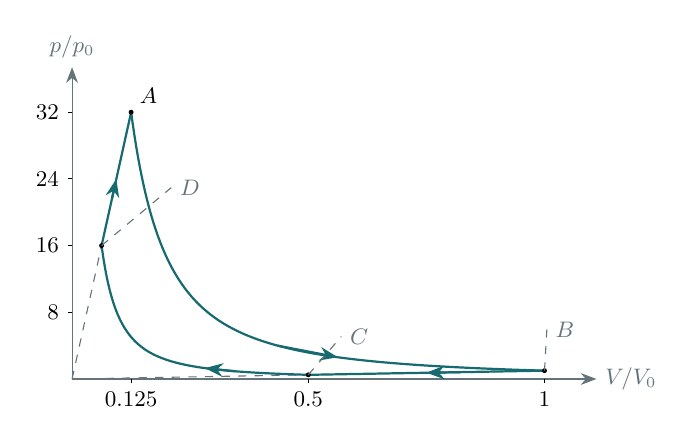
\begin{tikzpicture}[scale=.9,transform shape]
\draw[axis] (0,0)--(7.4,0) node[right] {$V/V_0$};
\draw[axis] (0,0)--(0,4.4) node[above] {$p/p_0$};
\draw[guide] (0,0)--(.8333333,3.7647059);
\draw[guide] (0,0)--(6.6666667,.1176471);
\draw[thin] (0.8333333,0)--(0.8333333,-.06) node[below] {$ 0.125 $};
\draw[thin] (3.3333333,0)--(3.3333333,-.06) node[below] {$ 0.5 $};
\draw[thin] (6.6666667,0)--(6.6666667,-.06) node[below] {$ 1 $};
\draw[thin] (0,0.9411765)--(-.06,0.9411765) node[left] {$ 8 $};
\draw[thin] (0,1.8823529)--(-.06,1.8823529) node[left] {$ 16 $};
\draw[thin] (0,2.8235294)--(-.06,2.8235294) node[left] {$ 24 $};
\draw[thin] (0,3.7647059)--(-.06,3.7647059) node[left] {$ 32 $};
\draw[traj] plot coordinates {(0.4166667,1.8823529) (0.4184028,1.8901961) (0.4201389,1.8980392) (0.4218750,1.9058824) (0.4236111,1.9137255) (0.4253472,1.9215686) (0.4270833,1.9294118) (0.4288194,1.9372549) (0.4305556,1.9450980) (0.4322917,1.9529412) (0.4340278,1.9607843) (0.4357639,1.9686275) (0.4375000,1.9764706) (0.4392361,1.9843137) (0.4409722,1.9921569) (0.4427083,2.0000000) (0.4444444,2.0078431) (0.4461806,2.0156863) (0.4479167,2.0235294) (0.4496528,2.0313725) (0.4513889,2.0392157) (0.4531250,2.0470588) (0.4548611,2.0549020) (0.4565972,2.0627451) (0.4583333,2.0705882) (0.4600694,2.0784314) (0.4618056,2.0862745) (0.4635417,2.0941176) (0.4652778,2.1019608) (0.4670139,2.1098039) (0.4687500,2.1176471) (0.4704861,2.1254902) (0.4722222,2.1333333) (0.4739583,2.1411765) (0.4756944,2.1490196) (0.4774306,2.1568627) (0.4791667,2.1647059) (0.4809028,2.1725490) (0.4826389,2.1803922) (0.4843750,2.1882353) (0.4861111,2.1960784) (0.4878472,2.2039216) (0.4895833,2.2117647) (0.4913194,2.2196078) (0.4930556,2.2274510) (0.4947917,2.2352941) (0.4965278,2.2431373) (0.4982639,2.2509804) (0.5000000,2.2588235) (0.5017361,2.2666667) (0.5034722,2.2745098) (0.5052083,2.2823529) (0.5069444,2.2901961) (0.5086806,2.2980392) (0.5104167,2.3058824) (0.5121528,2.3137255) (0.5138889,2.3215686) (0.5156250,2.3294118) (0.5173611,2.3372549) (0.5190972,2.3450980) (0.5208333,2.3529412) (0.5225694,2.3607843) (0.5243056,2.3686275) (0.5260417,2.3764706) (0.5277778,2.3843137) (0.5295139,2.3921569) (0.5312500,2.4000000) (0.5329861,2.4078431) (0.5347222,2.4156863) (0.5364583,2.4235294) (0.5381944,2.4313725) (0.5399306,2.4392157) (0.5416667,2.4470588) (0.5434028,2.4549020) (0.5451389,2.4627451) (0.5468750,2.4705882) (0.5486111,2.4784314) (0.5503472,2.4862745) (0.5520833,2.4941176) (0.5538194,2.5019608) (0.5555556,2.5098039) (0.5572917,2.5176471) (0.5590278,2.5254902) (0.5607639,2.5333333) (0.5625000,2.5411765) (0.5642361,2.5490196) (0.5659722,2.5568627) (0.5677083,2.5647059) (0.5694444,2.5725490) (0.5711806,2.5803922) (0.5729167,2.5882353) (0.5746528,2.5960784) (0.5763889,2.6039216) (0.5781250,2.6117647) (0.5798611,2.6196078) (0.5815972,2.6274510) (0.5833333,2.6352941) (0.5850694,2.6431373) (0.5868056,2.6509804) (0.5885417,2.6588235) (0.5902778,2.6666667) (0.5920139,2.6745098) (0.5937500,2.6823529) (0.5954861,2.6901961) (0.5972222,2.6980392) (0.5989583,2.7058824) (0.6006944,2.7137255) (0.6024306,2.7215686) (0.6041667,2.7294118) (0.6059028,2.7372549) (0.6076389,2.7450980) (0.6093750,2.7529412) (0.6111111,2.7607843) (0.6128472,2.7686275) (0.6145833,2.7764706) (0.6163194,2.7843137) (0.6180556,2.7921569) (0.6197917,2.8000000) (0.6215278,2.8078431) (0.6232639,2.8156863) (0.6250000,2.8235294) (0.6267361,2.8313725) (0.6284722,2.8392157) (0.6302083,2.8470588) (0.6319444,2.8549020) (0.6336806,2.8627451) (0.6354167,2.8705882) (0.6371528,2.8784314) (0.6388889,2.8862745) (0.6406250,2.8941176) (0.6423611,2.9019608) (0.6440972,2.9098039) (0.6458333,2.9176471) (0.6475694,2.9254902) (0.6493056,2.9333333) (0.6510417,2.9411765) (0.6527778,2.9490196) (0.6545139,2.9568627) (0.6562500,2.9647059) (0.6579861,2.9725490) (0.6597222,2.9803922) (0.6614583,2.9882353) (0.6631944,2.9960784) (0.6649306,3.0039216) (0.6666667,3.0117647) (0.6684028,3.0196078) (0.6701389,3.0274510) (0.6718750,3.0352941) (0.6736111,3.0431373) (0.6753472,3.0509804) (0.6770833,3.0588235) (0.6788194,3.0666667) (0.6805556,3.0745098) (0.6822917,3.0823529) (0.6840278,3.0901961) (0.6857639,3.0980392) (0.6875000,3.1058824) (0.6892361,3.1137255) (0.6909722,3.1215686) (0.6927083,3.1294118) (0.6944444,3.1372549) (0.6961806,3.1450980) (0.6979167,3.1529412) (0.6996528,3.1607843) (0.7013889,3.1686275) (0.7031250,3.1764706) (0.7048611,3.1843137) (0.7065972,3.1921569) (0.7083333,3.2000000) (0.7100694,3.2078431) (0.7118056,3.2156863) (0.7135417,3.2235294) (0.7152778,3.2313725) (0.7170139,3.2392157) (0.7187500,3.2470588) (0.7204861,3.2549020) (0.7222222,3.2627451) (0.7239583,3.2705882) (0.7256944,3.2784314) (0.7274306,3.2862745) (0.7291667,3.2941176) (0.7309028,3.3019608) (0.7326389,3.3098039) (0.7343750,3.3176471) (0.7361111,3.3254902) (0.7378472,3.3333333) (0.7395833,3.3411765) (0.7413194,3.3490196) (0.7430556,3.3568627) (0.7447917,3.3647059) (0.7465278,3.3725490) (0.7482639,3.3803922) (0.7500000,3.3882353) (0.7517361,3.3960784) (0.7534722,3.4039216) (0.7552083,3.4117647) (0.7569444,3.4196078) (0.7586806,3.4274510) (0.7604167,3.4352941) (0.7621528,3.4431373) (0.7638889,3.4509804) (0.7656250,3.4588235) (0.7673611,3.4666667) (0.7690972,3.4745098) (0.7708333,3.4823529) (0.7725694,3.4901961) (0.7743056,3.4980392) (0.7760417,3.5058824) (0.7777778,3.5137255) (0.7795139,3.5215686) (0.7812500,3.5294118) (0.7829861,3.5372549) (0.7847222,3.5450980) (0.7864583,3.5529412) (0.7881944,3.5607843) (0.7899306,3.5686275) (0.7916667,3.5764706) (0.7934028,3.5843137) (0.7951389,3.5921569) (0.7968750,3.6000000) (0.7986111,3.6078431) (0.8003472,3.6156863) (0.8020833,3.6235294) (0.8038194,3.6313725) (0.8055556,3.6392157) (0.8072917,3.6470588) (0.8090278,3.6549020) (0.8107639,3.6627451) (0.8125000,3.6705882) (0.8142361,3.6784314) (0.8159722,3.6862745) (0.8177083,3.6941176) (0.8194444,3.7019608) (0.8211806,3.7098039) (0.8229167,3.7176471) (0.8246528,3.7254902) (0.8263889,3.7333333) (0.8281250,3.7411765) (0.8298611,3.7490196) (0.8315972,3.7568627) (0.8333333,3.7647059)};
\draw[motion] (0.5642361,2.5490196)--(0.6250000,2.8235294);
\draw[traj] plot coordinates {(0.8333333,3.7647059) (0.8576389,3.5885709) (0.8819444,3.4252604) (0.9062500,3.2735246) (0.9305556,3.1322648) (0.9548611,3.0005115) (0.9791667,2.8774069) (1.0034722,2.7621890) (1.0277778,2.6541794) (1.0520833,2.5527723) (1.0763889,2.4574252) (1.1006944,2.3676510) (1.1250000,2.2830115) (1.1493056,2.2031114) (1.1736111,2.1275933) (1.1979167,2.0561334) (1.2222222,1.9884378) (1.2465278,1.9242391) (1.2708333,1.8632937) (1.2951389,1.8053791) (1.3194444,1.7502918) (1.3437500,1.6978455) (1.3680556,1.6478693) (1.3923611,1.6002058) (1.4166667,1.5547104) (1.4409722,1.5112499) (1.4652778,1.4697012) (1.4895833,1.4299504) (1.5138889,1.3918923) (1.5381944,1.3554294) (1.5625000,1.3204712) (1.5868056,1.2869335) (1.6111111,1.2547383) (1.6354167,1.2238127) (1.6597222,1.1940888) (1.6840278,1.1655034) (1.7083333,1.1379974) (1.7326389,1.1115156) (1.7569444,1.0860061) (1.7812500,1.0614206) (1.8055556,1.0377137) (1.8298611,1.0148428) (1.8541667,0.9927678) (1.8784722,0.9714513) (1.9027778,0.9508577) (1.9270833,0.9309538) (1.9513889,0.9117083) (1.9756944,0.8930916) (2.0000000,0.8750758) (2.0243056,0.8576344) (2.0486111,0.8407427) (2.0729167,0.8243771) (2.0972222,0.8085153) (2.1215278,0.7931362) (2.1458333,0.7782199) (2.1701389,0.7637474) (2.1944444,0.7497008) (2.2187500,0.7360631) (2.2430556,0.7228179) (2.2673611,0.7099501) (2.2916667,0.6974449) (2.3159722,0.6852884) (2.3402778,0.6734675) (2.3645833,0.6619694) (2.3888889,0.6507823) (2.4131944,0.6398946) (2.4375000,0.6292955) (2.4618056,0.6189745) (2.4861111,0.6089217) (2.5104167,0.5991276) (2.5347222,0.5895831) (2.5590278,0.5802796) (2.5833333,0.5712088) (2.6076389,0.5623628) (2.6319444,0.5537339) (2.6562500,0.5453149) (2.6805556,0.5370989) (2.7048611,0.5290792) (2.7291667,0.5212494) (2.7534722,0.5136033) (2.7777778,0.5061351) (2.8020833,0.4988392) (2.8263889,0.4917101) (2.8506944,0.4847426) (2.8750000,0.4779318) (2.8993056,0.4712728) (2.9236111,0.4647610) (2.9479167,0.4583919) (2.9722222,0.4521614) (2.9965278,0.4460653) (3.0208333,0.4400997) (3.0451389,0.4342606) (3.0694444,0.4285446) (3.0937500,0.4229480) (3.1180556,0.4174674) (3.1423611,0.4120996) (3.1666667,0.4068413) (3.1909722,0.4016896) (3.2152778,0.3966415) (3.2395833,0.3916941) (3.2638889,0.3868447) (3.2881944,0.3820907) (3.3125000,0.3774295) (3.3368056,0.3728586) (3.3611111,0.3683756) (3.3854167,0.3639782) (3.4097222,0.3596643) (3.4340278,0.3554315) (3.4583333,0.3512780) (3.4826389,0.3472015) (3.5069444,0.3432002) (3.5312500,0.3392721) (3.5555556,0.3354156) (3.5798611,0.3316286) (3.6041667,0.3279097) (3.6284722,0.3242570) (3.6527778,0.3206689) (3.6770833,0.3171440) (3.7013889,0.3136807) (3.7256944,0.3102775) (3.7500000,0.3069330) (3.7743056,0.3036458) (3.7986111,0.3004145) (3.8229167,0.2972379) (3.8472222,0.2941148) (3.8715278,0.2910438) (3.8958333,0.2880238) (3.9201389,0.2850536) (3.9444444,0.2821321) (3.9687500,0.2792583) (3.9930556,0.2764310) (4.0173611,0.2736492) (4.0416667,0.2709119) (4.0659722,0.2682182) (4.0902778,0.2655671) (4.1145833,0.2629577) (4.1388889,0.2603890) (4.1631944,0.2578603) (4.1875000,0.2553706) (4.2118056,0.2529192) (4.2361111,0.2505052) (4.2604167,0.2481279) (4.2847222,0.2457864) (4.3090278,0.2434801) (4.3333333,0.2412082) (4.3576389,0.2389701) (4.3819444,0.2367650) (4.4062500,0.2345923) (4.4305556,0.2324513) (4.4548611,0.2303414) (4.4791667,0.2282620) (4.5034722,0.2262124) (4.5277778,0.2241922) (4.5520833,0.2222006) (4.5763889,0.2202372) (4.6006944,0.2183015) (4.6250000,0.2163928) (4.6493056,0.2145106) (4.6736111,0.2126546) (4.6979167,0.2108240) (4.7222222,0.2090186) (4.7465278,0.2072378) (4.7708333,0.2054811) (4.7951389,0.2037481) (4.8194444,0.2020384) (4.8437500,0.2003516) (4.8680556,0.1986871) (4.8923611,0.1970447) (4.9166667,0.1954239) (4.9409722,0.1938243) (4.9652778,0.1922456) (4.9895833,0.1906873) (5.0138889,0.1891492) (5.0381944,0.1876308) (5.0625000,0.1861318) (5.0868056,0.1846519) (5.1111111,0.1831907) (5.1354167,0.1817479) (5.1597222,0.1803233) (5.1840278,0.1789164) (5.2083333,0.1775270) (5.2326389,0.1761548) (5.2569444,0.1747994) (5.2812500,0.1734607) (5.3055556,0.1721383) (5.3298611,0.1708320) (5.3541667,0.1695414) (5.3784722,0.1682664) (5.4027778,0.1670067) (5.4270833,0.1657619) (5.4513889,0.1645320) (5.4756944,0.1633166) (5.5000000,0.1621155) (5.5243056,0.1609284) (5.5486111,0.1597553) (5.5729167,0.1585957) (5.5972222,0.1574495) (5.6215278,0.1563166) (5.6458333,0.1551966) (5.6701389,0.1540894) (5.6944444,0.1529948) (5.7187500,0.1519126) (5.7430556,0.1508426) (5.7673611,0.1497846) (5.7916667,0.1487384) (5.8159722,0.1477038) (5.8402778,0.1466808) (5.8645833,0.1456690) (5.8888889,0.1446683) (5.9131944,0.1436786) (5.9375000,0.1426997) (5.9618056,0.1417314) (5.9861111,0.1407735) (6.0104167,0.1398260) (6.0347222,0.1388887) (6.0590278,0.1379613) (6.0833333,0.1370439) (6.1076389,0.1361361) (6.1319444,0.1352380) (6.1562500,0.1343492) (6.1805556,0.1334698) (6.2048611,0.1325996) (6.2291667,0.1317384) (6.2534722,0.1308861) (6.2777778,0.1300426) (6.3020833,0.1292078) (6.3263889,0.1283815) (6.3506944,0.1275637) (6.3750000,0.1267541) (6.3993056,0.1259527) (6.4236111,0.1251594) (6.4479167,0.1243741) (6.4722222,0.1235966) (6.4965278,0.1228269) (6.5208333,0.1220648) (6.5451389,0.1213103) (6.5694444,0.1205631) (6.5937500,0.1198234) (6.6180556,0.1190908) (6.6423611,0.1183654) (6.6666667,0.1176471)};
\draw[motion] (2.8993056,0.4712728)--(3.7500000,0.3069330);
\draw[traj] plot coordinates {(6.6666667,0.1176471) (6.6527778,0.1174020) (6.6388889,0.1171569) (6.6250000,0.1169118) (6.6111111,0.1166667) (6.5972222,0.1164216) (6.5833333,0.1161765) (6.5694444,0.1159314) (6.5555556,0.1156863) (6.5416667,0.1154412) (6.5277778,0.1151961) (6.5138889,0.1149510) (6.5000000,0.1147059) (6.4861111,0.1144608) (6.4722222,0.1142157) (6.4583333,0.1139706) (6.4444444,0.1137255) (6.4305556,0.1134804) (6.4166667,0.1132353) (6.4027778,0.1129902) (6.3888889,0.1127451) (6.3750000,0.1125000) (6.3611111,0.1122549) (6.3472222,0.1120098) (6.3333333,0.1117647) (6.3194444,0.1115196) (6.3055556,0.1112745) (6.2916667,0.1110294) (6.2777778,0.1107843) (6.2638889,0.1105392) (6.2500000,0.1102941) (6.2361111,0.1100490) (6.2222222,0.1098039) (6.2083333,0.1095588) (6.1944444,0.1093137) (6.1805556,0.1090686) (6.1666667,0.1088235) (6.1527778,0.1085784) (6.1388889,0.1083333) (6.1250000,0.1080882) (6.1111111,0.1078431) (6.0972222,0.1075980) (6.0833333,0.1073529) (6.0694444,0.1071078) (6.0555556,0.1068627) (6.0416667,0.1066176) (6.0277778,0.1063725) (6.0138889,0.1061275) (6.0000000,0.1058824) (5.9861111,0.1056373) (5.9722222,0.1053922) (5.9583333,0.1051471) (5.9444444,0.1049020) (5.9305556,0.1046569) (5.9166667,0.1044118) (5.9027778,0.1041667) (5.8888889,0.1039216) (5.8750000,0.1036765) (5.8611111,0.1034314) (5.8472222,0.1031863) (5.8333333,0.1029412) (5.8194444,0.1026961) (5.8055556,0.1024510) (5.7916667,0.1022059) (5.7777778,0.1019608) (5.7638889,0.1017157) (5.7500000,0.1014706) (5.7361111,0.1012255) (5.7222222,0.1009804) (5.7083333,0.1007353) (5.6944444,0.1004902) (5.6805556,0.1002451) (5.6666667,0.1000000) (5.6527778,0.0997549) (5.6388889,0.0995098) (5.6250000,0.0992647) (5.6111111,0.0990196) (5.5972222,0.0987745) (5.5833333,0.0985294) (5.5694444,0.0982843) (5.5555556,0.0980392) (5.5416667,0.0977941) (5.5277778,0.0975490) (5.5138889,0.0973039) (5.5000000,0.0970588) (5.4861111,0.0968137) (5.4722222,0.0965686) (5.4583333,0.0963235) (5.4444444,0.0960784) (5.4305556,0.0958333) (5.4166667,0.0955882) (5.4027778,0.0953431) (5.3888889,0.0950980) (5.3750000,0.0948529) (5.3611111,0.0946078) (5.3472222,0.0943627) (5.3333333,0.0941176) (5.3194444,0.0938725) (5.3055556,0.0936275) (5.2916667,0.0933824) (5.2777778,0.0931373) (5.2638889,0.0928922) (5.2500000,0.0926471) (5.2361111,0.0924020) (5.2222222,0.0921569) (5.2083333,0.0919118) (5.1944444,0.0916667) (5.1805556,0.0914216) (5.1666667,0.0911765) (5.1527778,0.0909314) (5.1388889,0.0906863) (5.1250000,0.0904412) (5.1111111,0.0901961) (5.0972222,0.0899510) (5.0833333,0.0897059) (5.0694444,0.0894608) (5.0555556,0.0892157) (5.0416667,0.0889706) (5.0277778,0.0887255) (5.0138889,0.0884804) (5.0000000,0.0882353) (4.9861111,0.0879902) (4.9722222,0.0877451) (4.9583333,0.0875000) (4.9444444,0.0872549) (4.9305556,0.0870098) (4.9166667,0.0867647) (4.9027778,0.0865196) (4.8888889,0.0862745) (4.8750000,0.0860294) (4.8611111,0.0857843) (4.8472222,0.0855392) (4.8333333,0.0852941) (4.8194444,0.0850490) (4.8055556,0.0848039) (4.7916667,0.0845588) (4.7777778,0.0843137) (4.7638889,0.0840686) (4.7500000,0.0838235) (4.7361111,0.0835784) (4.7222222,0.0833333) (4.7083333,0.0830882) (4.6944444,0.0828431) (4.6805556,0.0825980) (4.6666667,0.0823529) (4.6527778,0.0821078) (4.6388889,0.0818627) (4.6250000,0.0816176) (4.6111111,0.0813725) (4.5972222,0.0811275) (4.5833333,0.0808824) (4.5694444,0.0806373) (4.5555556,0.0803922) (4.5416667,0.0801471) (4.5277778,0.0799020) (4.5138889,0.0796569) (4.5000000,0.0794118) (4.4861111,0.0791667) (4.4722222,0.0789216) (4.4583333,0.0786765) (4.4444444,0.0784314) (4.4305556,0.0781863) (4.4166667,0.0779412) (4.4027778,0.0776961) (4.3888889,0.0774510) (4.3750000,0.0772059) (4.3611111,0.0769608) (4.3472222,0.0767157) (4.3333333,0.0764706) (4.3194444,0.0762255) (4.3055556,0.0759804) (4.2916667,0.0757353) (4.2777778,0.0754902) (4.2638889,0.0752451) (4.2500000,0.0750000) (4.2361111,0.0747549) (4.2222222,0.0745098) (4.2083333,0.0742647) (4.1944444,0.0740196) (4.1805556,0.0737745) (4.1666667,0.0735294) (4.1527778,0.0732843) (4.1388889,0.0730392) (4.1250000,0.0727941) (4.1111111,0.0725490) (4.0972222,0.0723039) (4.0833333,0.0720588) (4.0694444,0.0718137) (4.0555556,0.0715686) (4.0416667,0.0713235) (4.0277778,0.0710784) (4.0138889,0.0708333) (4.0000000,0.0705882) (3.9861111,0.0703431) (3.9722222,0.0700980) (3.9583333,0.0698529) (3.9444444,0.0696078) (3.9305556,0.0693627) (3.9166667,0.0691176) (3.9027778,0.0688725) (3.8888889,0.0686275) (3.8750000,0.0683824) (3.8611111,0.0681373) (3.8472222,0.0678922) (3.8333333,0.0676471) (3.8194444,0.0674020) (3.8055556,0.0671569) (3.7916667,0.0669118) (3.7777778,0.0666667) (3.7638889,0.0664216) (3.7500000,0.0661765) (3.7361111,0.0659314) (3.7222222,0.0656863) (3.7083333,0.0654412) (3.6944444,0.0651961) (3.6805556,0.0649510) (3.6666667,0.0647059) (3.6527778,0.0644608) (3.6388889,0.0642157) (3.6250000,0.0639706) (3.6111111,0.0637255) (3.5972222,0.0634804) (3.5833333,0.0632353) (3.5694444,0.0629902) (3.5555556,0.0627451) (3.5416667,0.0625000) (3.5277778,0.0622549) (3.5138889,0.0620098) (3.5000000,0.0617647) (3.4861111,0.0615196) (3.4722222,0.0612745) (3.4583333,0.0610294) (3.4444444,0.0607843) (3.4305556,0.0605392) (3.4166667,0.0602941) (3.4027778,0.0600490) (3.3888889,0.0598039) (3.3750000,0.0595588) (3.3611111,0.0593137) (3.3472222,0.0590686) (3.3333333,0.0588235)};
\draw[motion] (5.4861111,0.0968137)--(5.0000000,0.0882353);
\draw[traj] plot coordinates {(3.3333333,0.0588235) (3.3211806,0.0591827) (3.3090278,0.0595454) (3.2968750,0.0599117) (3.2847222,0.0602816) (3.2725694,0.0606551) (3.2604167,0.0610324) (3.2482639,0.0614134) (3.2361111,0.0617983) (3.2239583,0.0621870) (3.2118056,0.0625797) (3.1996528,0.0629764) (3.1875000,0.0633770) (3.1753472,0.0637818) (3.1631944,0.0641908) (3.1510417,0.0646039) (3.1388889,0.0650213) (3.1267361,0.0654431) (3.1145833,0.0658692) (3.1024306,0.0662998) (3.0902778,0.0667349) (3.0781250,0.0671746) (3.0659722,0.0676190) (3.0538194,0.0680681) (3.0416667,0.0685219) (3.0295139,0.0689807) (3.0173611,0.0694443) (3.0052083,0.0699130) (2.9930556,0.0703868) (2.9809028,0.0708657) (2.9687500,0.0713498) (2.9565972,0.0718393) (2.9444444,0.0723341) (2.9322917,0.0728345) (2.9201389,0.0733404) (2.9079861,0.0738519) (2.8958333,0.0743692) (2.8836806,0.0748923) (2.8715278,0.0754213) (2.8593750,0.0759563) (2.8472222,0.0764974) (2.8350694,0.0770447) (2.8229167,0.0775983) (2.8107639,0.0781583) (2.7986111,0.0787248) (2.7864583,0.0792978) (2.7743056,0.0798776) (2.7621528,0.0804642) (2.7500000,0.0810577) (2.7378472,0.0816583) (2.7256944,0.0822660) (2.7135417,0.0828810) (2.7013889,0.0835033) (2.6892361,0.0841332) (2.6770833,0.0847707) (2.6649306,0.0854160) (2.6527778,0.0860692) (2.6406250,0.0867304) (2.6284722,0.0873997) (2.6163194,0.0880774) (2.6041667,0.0887635) (2.5920139,0.0894582) (2.5798611,0.0901616) (2.5677083,0.0908740) (2.5555556,0.0915954) (2.5434028,0.0923259) (2.5312500,0.0930659) (2.5190972,0.0938154) (2.5069444,0.0945746) (2.4947917,0.0953437) (2.4826389,0.0961228) (2.4704861,0.0969122) (2.4583333,0.0977120) (2.4461806,0.0985224) (2.4340278,0.0993436) (2.4218750,0.1001758) (2.4097222,0.1010192) (2.3975694,0.1018741) (2.3854167,0.1027406) (2.3732639,0.1036189) (2.3611111,0.1045093) (2.3489583,0.1054120) (2.3368056,0.1063273) (2.3246528,0.1072553) (2.3125000,0.1081964) (2.3003472,0.1091507) (2.2881944,0.1101186) (2.2760417,0.1111003) (2.2638889,0.1120961) (2.2517361,0.1131062) (2.2395833,0.1141310) (2.2274306,0.1151707) (2.2152778,0.1162257) (2.2031250,0.1172961) (2.1909722,0.1183825) (2.1788194,0.1194851) (2.1666667,0.1206041) (2.1545139,0.1217401) (2.1423611,0.1228932) (2.1302083,0.1240639) (2.1180556,0.1252526) (2.1059028,0.1264596) (2.0937500,0.1276853) (2.0815972,0.1289302) (2.0694444,0.1301945) (2.0572917,0.1314788) (2.0451389,0.1327836) (2.0329861,0.1341091) (2.0208333,0.1354560) (2.0086806,0.1368246) (1.9965278,0.1382155) (1.9843750,0.1396291) (1.9722222,0.1410661) (1.9600694,0.1425268) (1.9479167,0.1440119) (1.9357639,0.1455219) (1.9236111,0.1470574) (1.9114583,0.1486190) (1.8993056,0.1502073) (1.8871528,0.1518229) (1.8750000,0.1534665) (1.8628472,0.1551387) (1.8506944,0.1568403) (1.8385417,0.1585720) (1.8263889,0.1603345) (1.8142361,0.1621285) (1.8020833,0.1639548) (1.7899306,0.1658143) (1.7777778,0.1677078) (1.7656250,0.1696361) (1.7534722,0.1716001) (1.7413194,0.1736007) (1.7291667,0.1756390) (1.7170139,0.1777158) (1.7048611,0.1798321) (1.6927083,0.1819891) (1.6805556,0.1841878) (1.6684028,0.1864293) (1.6562500,0.1887147) (1.6440972,0.1910454) (1.6319444,0.1934224) (1.6197917,0.1958471) (1.6076389,0.1983207) (1.5954861,0.2008448) (1.5833333,0.2034207) (1.5711806,0.2060498) (1.5590278,0.2087337) (1.5468750,0.2114740) (1.5347222,0.2142723) (1.5225694,0.2171303) (1.5104167,0.2200498) (1.4982639,0.2230327) (1.4861111,0.2260807) (1.4739583,0.2291960) (1.4618056,0.2323805) (1.4496528,0.2356364) (1.4375000,0.2389659) (1.4253472,0.2423713) (1.4131944,0.2458550) (1.4010417,0.2494196) (1.3888889,0.2530676) (1.3767361,0.2568017) (1.3645833,0.2606247) (1.3524306,0.2645396) (1.3402778,0.2685495) (1.3281250,0.2726575) (1.3159722,0.2768670) (1.3038194,0.2811814) (1.2916667,0.2856044) (1.2795139,0.2901398) (1.2673611,0.2947915) (1.2552083,0.2995638) (1.2430556,0.3044608) (1.2309028,0.3094872) (1.2187500,0.3146477) (1.2065972,0.3199473) (1.1944444,0.3253911) (1.1822917,0.3309847) (1.1701389,0.3367337) (1.1579861,0.3426442) (1.1458333,0.3487224) (1.1336806,0.3549750) (1.1215278,0.3614090) (1.1093750,0.3680315) (1.0972222,0.3748504) (1.0850694,0.3818737) (1.0729167,0.3891099) (1.0607639,0.3965681) (1.0486111,0.4042576) (1.0364583,0.4121885) (1.0243056,0.4203713) (1.0121528,0.4288172) (1.0000000,0.4375379) (0.9878472,0.4465458) (0.9756944,0.4558542) (0.9635417,0.4654769) (0.9513889,0.4754288) (0.9392361,0.4857256) (0.9270833,0.4963839) (0.9149306,0.5074214) (0.9027778,0.5188568) (0.8906250,0.5307103) (0.8784722,0.5430030) (0.8663194,0.5557578) (0.8541667,0.5689987) (0.8420139,0.5827517) (0.8298611,0.5970444) (0.8177083,0.6119063) (0.8055556,0.6273691) (0.7934028,0.6434668) (0.7812500,0.6602356) (0.7690972,0.6777147) (0.7569444,0.6959462) (0.7447917,0.7149752) (0.7326389,0.7348506) (0.7204861,0.7556250) (0.7083333,0.7773552) (0.6961806,0.8001029) (0.6840278,0.8239346) (0.6718750,0.8489228) (0.6597222,0.8751459) (0.6475694,0.9026895) (0.6354167,0.9316468) (0.6232639,0.9621196) (0.6111111,0.9942189) (0.5989583,1.0280667) (0.5868056,1.0637967) (0.5746528,1.1015557) (0.5625000,1.1415058) (0.5503472,1.1838255) (0.5381944,1.2287126) (0.5260417,1.2763861) (0.5138889,1.3270897) (0.5017361,1.3810945) (0.4895833,1.4387034) (0.4774306,1.5002558) (0.4652778,1.5661324) (0.4531250,1.6367623) (0.4409722,1.7126302) (0.4288194,1.7942855) (0.4166667,1.8823529)};
\draw[motion] (2.3003472,0.1091507)--(1.8750000,0.1534665);
\fill (0.8333333,3.7647059) circle(.035);
\node[above right] at (0.8333333,3.7647059) {$A$};
\fill (6.6666667,0.1176471) circle(.035);
\draw[guide] (6.6666667,0.1176471)--(6.7,0.7) node[right] {$B$};
\fill (3.3333333,0.0588235) circle(.035);
\draw[guide] (3.3333333,0.0588235)--(3.8,0.6) node[right] {$C$};
\fill (0.4166667,1.8823529) circle(.035);
\draw[guide] (0.4166667,1.8823529)--(1.4,2.7) node[right] {$D$};
\end{tikzpicture}
\figcaption{图热试1.2\quad 第2问归一化压强体积循环，$p_0=RT_0/V_0$}
\end{minipage}\end{center}

\par\vspace{5mm}\noindent{\small\color{muted}作答区}\par\vspace{3mm}\noindent\textcolor{rulegray}{\rule{\linewidth}{0.3pt}}\par\vspace{12mm}\noindent\textcolor{rulegray}{\rule{\linewidth}{0.3pt}}

\clearpage

\pdfbookmark[2]{第 3 题 绝热大气分层与高速物体的碰撞阻力}{q3}

\section*{第 3 题\quad 绝热大气分层与高速物体的碰撞阻力}\label{q:3}


把近地大气视为理想气体，氮、氧分子的数目比例为$4:1$。一小团近地空气缓慢上升时与周围换热可忽略；以各层都处于这一干绝热分层的近似计算。地面温度取$T_0=300\ \mathrm K$（约$27^\circ\mathrm C$），压强$p_0=1.01\times10^5\ \mathrm{Pa}$。
\begin{enumerate}
\item 求$h=10\ \mathrm{km}$处的温度，并求当地压强与密度供下一问使用。
\item 截面积$A=1\ \mathrm{m^2}$的球形物体位于该高度，初速度恰等于没有大气时的圆轨道速度。为估算初始阻力，按如下简化：所有撞到垂直于运动方向截面的分子都与该截面发生弹性正碰，物体速度在单次分子碰撞中可视为不变；忽略分子热运动。估算阻力大小，说明忽略热运动的依据。
\end{enumerate}
取$g=9.8\ \mathrm{m\,s^{-2}}$为常量，地球半径$R_E=6.4\times10^6\ \mathrm m$，
$R=8.31\ \mathrm{J\,mol^{-1}K^{-1}}$，氮、氧的摩尔质量分别为$0.028,0.032\ \mathrm{kg\,mol^{-1}}$。


\begin{center}\begin{minipage}{.98\linewidth}\centering
\begin{tikzpicture}[scale=.9,transform shape]

\fill[accent!8] (0,0) rectangle (5,3.4);
\draw[object] (-.3,0)--(5.5,0);\node[below] at (2.5,0) {地面 $T_0,p_0$};
\draw[axis] (-.4,0)--(-.4,4) node[above] {$z$};
\draw[guide] (0,3)--(5,3);\node[right] at (5,3) {$h=10\ \mathrm{km}$};
\draw[object] (1.2,1.2) rectangle (3.4,1.65);
\node at (2.3,1.43) {薄层};
\draw[axis,<->] (3.65,1.2)--(3.65,1.65) node[midway,right] {$\mathrm dz$};
\draw[force] (1.65,.6)--(1.65,1.18) node[below left] {$pA_z$};
\draw[force] (2.9,2.3)--(2.9,1.68) node[above left] {$(p+\mathrm dp)A_z$};
\draw[force] (2.3,1.2)--(2.3,.5) node[below] {$\rho gA_z\,\mathrm dz$};
\draw[motion] (4.1,2.5)--(4.1,3.5) node[above] {空气团};

\end{tikzpicture}
\figcaption{图热试1.3\quad 薄层静力平衡与缓慢绝热上升空气团。}
\end{minipage}\end{center}

\par\vspace{5mm}\noindent{\small\color{muted}作答区}\par\vspace{3mm}\noindent\textcolor{rulegray}{\rule{\linewidth}{0.3pt}}\par\vspace{12mm}\noindent\textcolor{rulegray}{\rule{\linewidth}{0.3pt}}

\clearpage

\pdfbookmark[2]{第 4 题 有限热容量物体之间的温差衰减}{q4}

\section*{第 4 题\quad 有限热容量物体之间的温差衰减}\label{q:4}


热容量分别为$C_1,C_2>0$的两金属块用一根热容量可忽略的粗棒连接，整体与外界绝热。每块内部温度均匀，棒传热功率与两块温度差成正比：
\[
\dot Q_{1\to2}=\kappa(\tau_1-\tau_2),\qquad \kappa>0.
\]
$t=0$时两块的温度分别为$\tau_{10},\tau_{20}$。求温差大小降到初始大小一半所需时间，以及该时刻两块的温度。另说明初始温度相等时如何理解这一问。


\begin{center}\begin{minipage}{.98\linewidth}\centering
\begin{tikzpicture}[scale=.9,transform shape]

\draw[object,fill=warm!8] (0,0) rectangle (2,1.6);
\draw[object,fill=accent!8] (5,0) rectangle (7,1.6);
\draw[object,fill=muted!10] (2,.65) rectangle (5,.95);
\node[align=center] at (1,.8) {$A$\\$C_1,\tau_1$};
\node[align=center] at (6,.8) {$B$\\$C_2,\tau_2$};
\draw[force] (2.5,1.3)--(4.5,1.3) node[midway,above] {$\dot Q_{1\to2}=\kappa(\tau_1-\tau_2)$};
\draw[guide,rounded corners] (-.35,-.35) rectangle (7.35,2.2);
\node[below] at (3.5,-.4) {整体绝热；棒不蓄热};

\end{tikzpicture}
\figcaption{图热试1.4\quad 热流正方向取A到B，代数温差决定实际方向。}
\end{minipage}\end{center}

\workarea

\clearpage

\pdfbookmark[2]{第 5 题 晶体的非谐势能与热膨胀参数}{q5}

\section*{第 5 题\quad 晶体的非谐势能与热膨胀参数}\label{q:5}


含$N$对正负离子的NaCl晶体，相互作用总势能用
\[
E_p(r)=N\left(\frac{a_m}{r^m}-\frac{\alpha e^2}{4\pi\varepsilon_0r}\right)
\]
描述。$r$为最近邻正、负离子间距，$r_0$为零压平衡间距；$a_m,\alpha>0$，$m>1$为待定排斥指数，拟合时允许为实数。记平衡势能为$E_{p0}$，相对偏移$x=(r-r_0)/r_0$，并展开
\[
U(x)=E_p-E_{p0}=A_0+A_1x+A_2x^2+A_3x^3+\cdots.
\]
给定经典小振动统计关系
\[
\langle x\rangle=CT,\qquad
C=-\frac{3NkA_3}{4A_2^2}.
\]
\begin{enumerate}
\item 求$A_0,A_1,A_2,A_3$与$m,\alpha,r_0$的关系，并说明非零热膨胀的成因。
\item 已测$r_0=2.81\times10^{-10}\ \mathrm m$、
$C=7.65\times10^{-6}\ \mathrm{K^{-1}}$，平衡附近绝热压缩系数
\[
\kappa_s=-\frac1V\left(\frac{\mathrm dV}{\mathrm dp}\right)_s
=3.3\times10^{-11}\ \mathrm{Pa^{-1}}.
\]
按静态晶格势能主导弹性响应的近似，求$m,\alpha,a_m$。NaCl常规立方晶胞边长为$2r$、每胞含4对离子。讨论把$m$限定为整数以及提前舍入$m$对$a_m$表示的影响。
\end{enumerate}
取$e=1.60\times10^{-19}\ \mathrm C$、$\varepsilon_0=8.90\times10^{-12}\ \mathrm{F/m}$、
$k=1.38\times10^{-23}\ \mathrm{J/K}$。


\begin{center}\begin{minipage}{.98\linewidth}\centering
\begin{tikzpicture}[scale=.9,transform shape]

\foreach \i in {0,1,2} {\foreach \j in {0,1,2} {
\pgfmathtruncatemacro{\sgn}{mod(\i+\j,2)}
\ifnum\sgn=0 \draw[object,fill=accent!10] (\i*1.3,\j*1.3) circle (.17) node {$+$};
\else \draw[object,fill=warm!10] (\i*1.3,\j*1.3) circle (.17) node {$-$};\fi}}
\draw[guide] (0,0)--(2.6,0)--(2.6,2.6)--(0,2.6)--cycle;
\draw[axis,<->] (0,-.55)--(1.3,-.55) node[midway,below] {$r$};
\draw[axis,<->] (0,3.15)--(2.6,3.15) node[midway,above] {$2r$};
\node[right,align=left] at (3.3,1.6) {晶胞的一层截面\\[5pt]立方晶胞含4对离子\\[5pt]$V=(N/4)(2r)^3$};

\end{tikzpicture}
\figcaption{图热试1.5\quad 最近邻距离与常规晶胞边长；正负号表示离子电荷。}
\end{minipage}\end{center}

\par\vspace{5mm}\noindent{\small\color{muted}作答区}\par\vspace{3mm}\noindent\textcolor{rulegray}{\rule{\linewidth}{0.3pt}}\par\vspace{12mm}\noindent\textcolor{rulegray}{\rule{\linewidth}{0.3pt}}

\end{document}
